\documentclass{beamer}

%For 16:10 screens/projectors
%\usepackage[orientation=landscape,size=custom,width=16,height=10,scale=0.5,debug]{beamerposter} 

\mode<presentation>
{
  \usetheme{Madrid}
  \setbeamercovered{transparent}
}
%\useoutertheme{infolines}


\usepackage[english]{babel}
\usepackage[latin1]{inputenc}
\usepackage{amsmath}
\usepackage{multimedia}
\usepackage{pgf}
\usepackage{pst-gantt}
\usepackage{graphicx,color,psfrag}
\DeclareGraphicsExtensions{.png,.jpg}
\usepackage{pstricks}
\usepackage{epsf,multirow,textcomp}
\usepackage{algorithm,algorithmic}
\usepackage{epstopdf}
%\usepackage{enumitem}


\title[Feature Learning with Neural Nets]{\Large{Improved Music Feature Learning with Deep Neural Networks} }

\author[S. Sigtia and S. Dixon]{Siddharth Sigtia and Simon Dixon\\ \texttt{\scriptsize{\{sss31,simond\}@qmul.ac.uk}}}

\institute[C4DM]{Centre for Digital Music\\Queen Mary University of London}

\date{}

%Left logo
\pgfdeclareimage[height=0.4cm]{c4dm}{Figures/cd4m.eps}
\setbeamertemplate{sidebar left}{
   \vfill
   \rlap{\hskip0.1cm \href{http://www.elec.qmul.ac.uk/digitalmusic/index.html}{\pgfuseimage{c4dm}}}
   \vskip2pt
   \llap{\usebeamertemplate***{navigation symbols}\hskip0.1cm}
   \vskip2pt
} 

%Right logo
\logo{
\includegraphics[height=0.5cm]{Figures/qm_blue_logo.eps}}


\begin{document}

\begin{frame}
  \titlepage
\end{frame}


\section{Introduction}


\begin{frame}{Motivation}
\vspace{-0.15in}
  \begin{itemize}
  \item Try to learn the most optimal features for a particular task and reduce dependency on hand-crafted features.
  \item {\usebeamercolor[fg]{structure} How can we learn features for a particular task?}:
    \\Neural nets with several hidden layers (deep neural networks).  
  \item {\usebeamercolor[fg]{structure} Can we learn features for MIR tasks with neural nets?}: 
    \\Lots of recent evidence suggests yes!     
  \end{itemize}
\end{frame}


\begin{frame}{Challenges with this approach?}
%{\usebeamercolor[fg]{structure}Optimisation}
  \begin{itemize}
    \item Optimising networks with several hidden layers is challenging. 
    \item The error surface is highly non-linear w.r.t. parameters and the best we can do is hope to find a useful local minimum. 
    \item The number of hyper-parameters can be quite large if we include momentum, learning rate schedules etc.   
    \item For large networks, Stochastic Gradient Descent (SGD) can take prohibitively long to find useful minima even with unsupervised pre-training. 
    \item In several domains (including music/audio), it is quite important to understand/interpret the learnt features. Something that is not clear with deep neural nets. 
  \end{itemize}
\end{frame}

\begin{frame}{Can we do better?}
  \begin{itemize}
    \item The use of neural networks for supervised learning has come full circle in some ways.
    \item Unsupervised pre-training is not considered to be necessary for finding good solutions. 
    \item Gradient based optimisers starting with random parameter initialisation provide good results. 
    \item Rectified Linear Units (ReLUs), Dropout, Hessian Free (HF) optimisation, Nesterov's Accelerated Gradient have all been applied to problems in various domains.
    \item The application of these new techniques to learning features for MIR tasks could provide improvements over existing methods.  
  \end{itemize}
\end{frame}

\begin{frame}{Problem definition}
  \begin{itemize}
    \item Learn features for a genre classification task using data from the GTZAN dataset.
    \item Train a classifier on the learned features and evaluate system performance.
    \item Inspect if features are general by using the same features on the ISMIR2004 genre dataset. 
  \end{itemize}
  This area will contain a diagram of the general pipeline
\end{frame}

\begin{frame}{Contributions Of The Paper}
{\usebeamercolor[fg]{structure} Whats different?}
\begin{itemize}
    \item Evaluate the use of ReLUs as hidden units.
    \item Use Dropout for regularisation.
    \item Use HF Optimisation for training sigmoid nets and compare. 
  \end{itemize}
{\usebeamercolor[fg]{structure} Hypothesis?}
\begin{itemize}
    \item ReLUs+Dropout eliminate the need for pre-training.
    \item Performance(ReLU+Dropout+SGD) $>=$ Performance(sigmoid nets+SGD)
    \item More efficient training of sigmoid nets with HF.
  \end{itemize}
\end{frame}

\begin{frame}{Feature Extraction}
This slide is going to contain a pictorial representation of the feature extraction. 
\end{frame}

\begin{frame}{Rectified Linear Units}
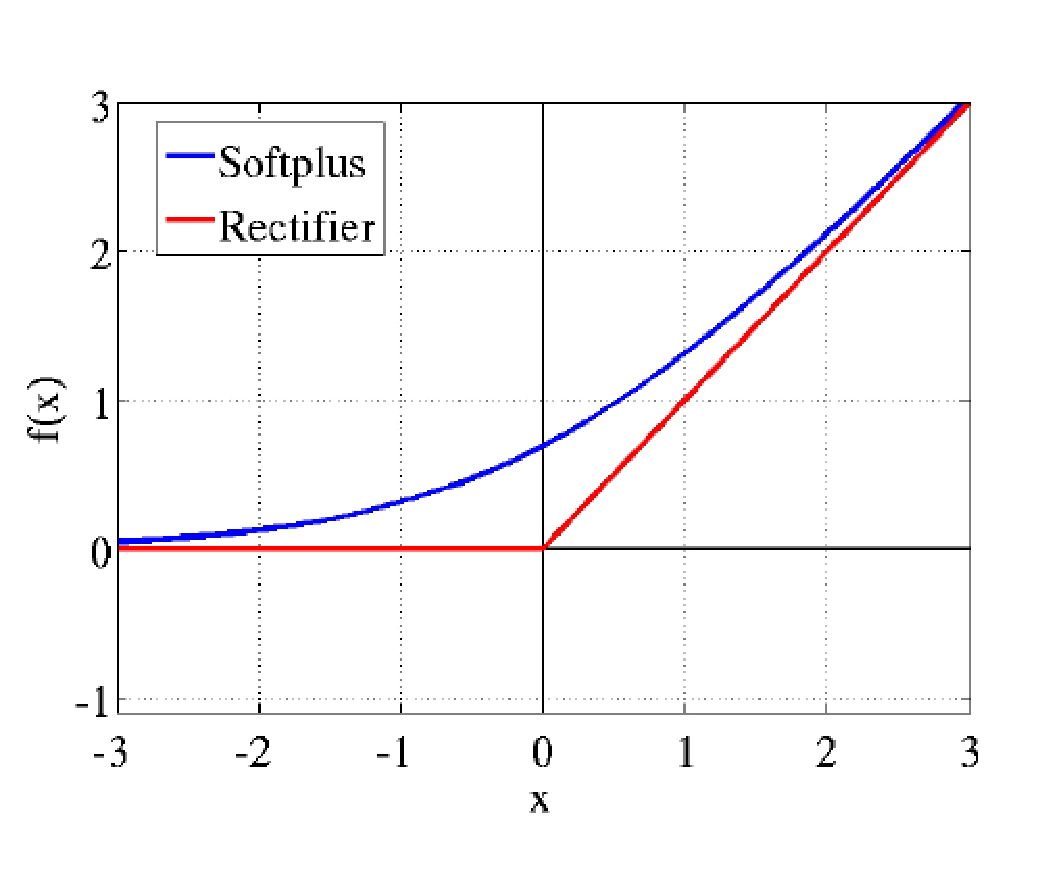
\includegraphics[scale=0.3]{Figures/ReLU-acts.eps}
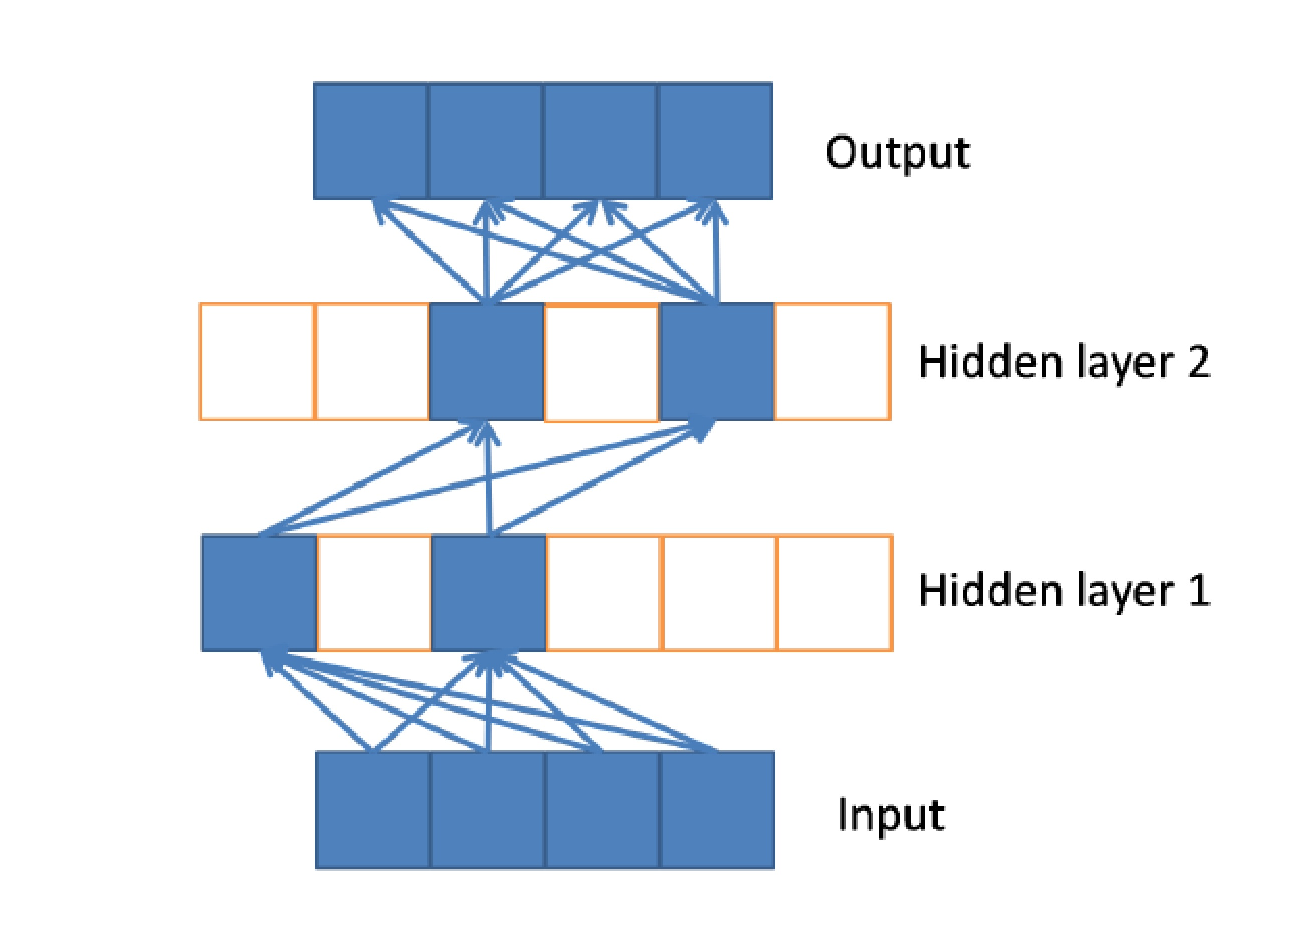
\includegraphics[scale=0.3]{Figures/ReLU-grads.eps}
\\
Activation function: $f(x) = max(0,x)$
\end{frame}

\begin{frame}{Dropout}
{\usebeamercolor[fg]{structure} Training}
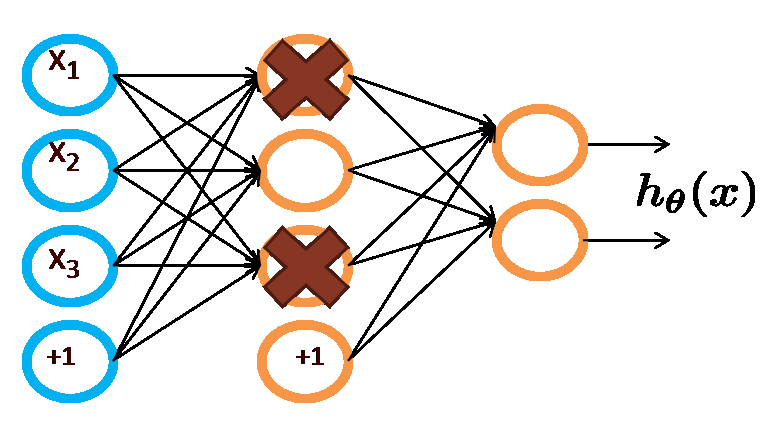
\includegraphics[scale=0.5]{Figures/dropout.eps}
{\usebeamercolor[fg]{structure} Forward Propagation}
$$y^{l} = \frac{1}{1-p}W^{l}(r^{l-1} * y^{l-1} + b^{l})$$
\end{frame}

\begin{frame}{Useful Properties of ReLUs}
\begin{itemize}
    \item No need for supervised pre-training.
    \item Hard sparsity in hidden layers.
    \item Gradients flow easily.
    \item Error surface is less convoluted w.r.t parameters because of the form of the activation function.
  \end{itemize}
\end{frame}


\end{document}



